\documentclass[12pt, preprint]{aastex}
\usepackage{graphicx}	% For figures
\usepackage{natbib}	% For citep and citep
\usepackage{amsmath}	% for \iint
\usepackage{bbm}
\usepackage[breaklinks]{hyperref}	% for blackboard bold numbers
\usepackage{hyperref}
\hypersetup{colorlinks}
\usepackage{color}
\usepackage{morefloats}
\definecolor{darkred}{rgb}{0.5,0,0}
\definecolor{darkgreen}{rgb}{0,0.5,0}
\definecolor{darkblue}{rgb}{0,0,0.5}
\hypersetup{ colorlinks,
linkcolor=darkblue,
filecolor=darkgreen,
urlcolor=darkred,
citecolor=darkblue }


\newcommand{\beq}{\begin{equation}}
\newcommand{\eeq}{\end{equation}}

\begin{document}

\author{
  Mohammadjavad~Vakili\altaffilmark{1},
  David~W.~Hogg\altaffilmark{1,2,3}
\altaffiltext{1}{Center for Cosmology and Particle Physics, New York University}
\altaffiltext{2}{Center for Data Science, New York University}
\altaffiltext{3}{Max-Planck-Institut f\"ur Astronomie}
}

\title{Fast and optimal centroiding of faint stars}

\begin{abstract}

One of the most demanding tasks in astronomical image processing is centroiding of stars. 
The upcoming large scale astronomical surveys are going to take images of billions of point sources, 
including many faint stars, in short exposure times. Thus, real-time accurate estimation of the
centroid of stars is crucial for further analysis of the photometric data such as PSF estimation,
and infering the proper motion of stars. In this work, we aim to compare the performances of
fast and profile-fitting centroiding methods when applied to relatively low signal-to-noise ratio
stars in a wide range of full width at half maxima.
Besides, in order to see how information preserving these techniques are, we compare
the root-mean-squared-error arising from these centroiding techniques with the Cramer-Rao
lower bound. The methods we discuss in this paper are: the naive 3$\times$3 polynomial centroiding,
a modification of this method, 3$\times$3 quartic approximation, and PSF profile fitting.
We find that 3$\times$3 modified polynomial cetroiding leads to
significant improvement in comparison with the naive polynomial centroiding, and gives rise
to centroiding errors comparable to those of 3$\times$3 quartic approximation method.
Moreover, our findings suggest that the 3$\times$3 modified polynomial, and the 3$\times$3
quartic approximation techniques, though not as accurate as PSF profile fitting methods,
are able to deliver results sufficiently close to saturating the Cramer-Rao lower bound in a range 
of relatively faint stars.

\end{abstract}

\section{Introduction}

A common practice in astronomy is taking imaging data, and then finding the coordinates
of various light sources across the sky. Finding accuarate estimate of the center of point
sources, convolved with telescope point spread function (and atmospheric PSF in case of
ground based telescopes), and also pixel response function, is crucial to further steps of
astronomical image processing. For instance, proper measurement of the shapes of galaxies
requires interpolating the PSF from the position of sparsely located stars across the
image to the positions of galaxies. The accuracy of the PSF estimation therefore,
relies on how accurately we know the centroid of stars. 

Ideally, we want a centroiding procedure that provides measurements as accurate as possible,
without putting a huge computational burden on the photometric pipeline.
Reducing the computational cost becomes even more important in large surveys,
where we want to estimate the centroid of thousands of point sources detected
on the telescope's focal plane. 

Reaching the optimal measurement of the centroid of stars however, is limited
by the lack of knowledge about the exact shape of the PSF, and also presence of noise;
both sky noise and CCD readout noise. Thus, of particular interest is devising a fast method that returns
optimal estimates of centroids in a realistic range of signal-to-noise ratios.

To date, a number of softwares have been designed for the purpose of extracting astronomical
sources and making catalogs. One of these softwares is SExtractor \citep{sex},
whose centroiding method involves first, finding the zeroth moment of the object
as a first-order estimate, and then iteratively correcting the centroid by computing
the zeroth order moment of the object weighted by a Gaussian window function,
until the correction falls below a particular threshold value.
The width of the Gaussian window function is set by the object's half light radius.

Another examples are DAOPHOT \citep{daophot}, and DOPHOT \citep{dophot}
which both assume analytic models for the stellar PSF profiles with centroid
coordinates being free parameters of these models.
DAOPHOT (DoPHOT) finds the centroid by fitting a Gaussian (power law) PSF to
the light profile of stars.

In this paper, we propose to find the centroid of stars by smoothing the image
of stars by a Gaussian kernel, and fitting a second order polynomial to
the $3\times$3 pixels around the brightest pixel of smoothed image.
We compare the accuracy of this method with, the naive 3$\times$3 second-order 
polynomial method, the 3$\times$3 quartic approximation
method used in SDSS photometric pipeline, and fitting a PSF model to the 
star.

In order to do so, we apply these methods to a large number of simulated
stars with different signal-to-noise ratio and size realizations. 
Error from star centroiding methods, will always have 
a theoretically-set lower bound, known as the Cramer-Rao lower bound
(hereafter denoted by CRLB) which has an inverse relation with the
signal-to-noise-ratio of stars.

Given the analytic model for the PSF,
we derive an expression for CRLB on the centroiding error as
a function of the parameters of the PSF model (\eg FWHM),
and signal-to-noise-ratio of stars. We create two sets of simulations for which we 
know the CRLB, one with variable (constant) signal-to-noise ratio (FWHM), and one 
with variable (constant) FWHM (signal-to-noise ratio). After applying
different centroiding methods to the simulations,
we investigate how close these methods can get to saturating the CRLB for
various ranges of background noise and FWHM.

This paper is structured as follows. In section \ref{sec:method},
we give a brief overview of the centroiding methods used in our investigation.
In section \ref{sec:data}, we discuss the simulated data, and the CRLB on centroiding error.
In section \ref{sec:results}, we compare the results of our proposed method with 
those obtained from centroiding methods discussed in \ref{sec:method}, and 
with the CRLB derived in \ref{sec:data}. Finally, we discuss and conclude
in \ref{sec:discussion}.               

\section{Methods}\label{sec:method}

\subsection{3$\times$3 polynomial method}

In order to find the centroid of a star, 
we fit a simple 2d polynomial $P(x,y)=a+bx+cy+dx^2+exy+fy^2$ to the
$3\times3$ patch centered on the brightest pixel of the
image. We apply this method to star images in the sky-dominated regime.
In this regime, the covariance matrix of pixel uncertianties is simply
given by $\sigma^{2}\mathbf{I}$, where $\sigma^{2}$ is variance of the
uncorrelated Gaussian noise, and $\mathbf{I}$ is a 9$\times$9 identity matrix.
Upon constructing a universal 9$\times$6 design matrix
\begin{equation}
    \mathbf{A} = 
    \begin{bmatrix}
        1 & x_{1} & y_{1} & x_{1}^{2} & x_{1}y_{1} & y_{1}^{2} \\
        . & . & . & . & . & .  \\
        . & . & . & . & . & .  \\
        . & . & . & . & . & .  \\
        1 & x_{9} & y_{9} & x_{9}^{2} & x_{9}y_{9} & y_{9}^{2}
    \end{bmatrix},
\end{equation}
the free parameters of the model $\{a,b,c,d,e,f\}$
(hereafter compactly denoted by $\mathbf{X}$) can be determined by 
\beq
\mathbf{X} = (\mathbf{A}^{T}\mathbf{A})^{-1}\mathbf{A}^{T}\mathbf{Z},
\label{linearfit}
\eeq
where $\mathbf{Z}$ is given by $(z_{1},...,z_{9})^{T}$,
with $z_{i}$, being the brightness of the $i-$th pixel of the 3$\times$3 patch.
Afterwards, the best fit parameters can be used to compute the centroid coordinate

\beq
  \begin{bmatrix}
      x_{c}\\
      y_{c}\\
  \end{bmatrix} = 
  \begin{bmatrix}
      2d & e\\
      e & 2f\\
  \end{bmatrix}^{-1}
  \begin{bmatrix}
      -b\\
      -c\\
  \end{bmatrix}.
\label{center}
\eeq

It is important to note that the algebraic operation in (\ref{center}) involves 
inverting a 2$\times$2 curvature matrix
\beq
  D = 
  \begin{bmatrix}
      2d & e\\
      e & 2f\\
  \end{bmatrix}.
\eeq
When D has a zero (or very close to zero) deteminant,
centroid estimated by (\ref{center}) gets arbitrarily 
large in which case the centroiding method leads to a catastrophic 
outlier. In order to tackle this issue, we add a small regularization term
proportional to $\sigma$ to the diagonal elements of the curvature matrix.
This soft regularization term prevents the determinant of the curvature matrix from
getting zero, and removes the catastrophic outliers.

\subsection{3$\times$3 modified polynomial method}
Now, we modify the simple polynomial method explained above,
by smoothing the image of the star with a Gaussian kernel
\beq
k(\mathbf{x}) = \frac{1}{2\pi w^2}\exp(-\mathbf{x}^{2}/2w^{2}).
\eeq
Throughout this study, we keep the width of the Gaussian kernel $w$ constant.
Then we apply the same polynomial method to the 3$\times$3 patch around the brightest
pixel of the smoothed image. The important difference between the previous
approach and the modified method is that, there are non-zero covariances
among the uncertainties of the brightness of different pixels of the
smoothed image. That is, the covariance matrix $\mathbf{C}$ is non-diagonal.
It can be shown that after smoothing, elements of the covariance matrix are given by
\begin{eqnarray}
\mathbf{C}_{ij} &=& \frac{\sigma^{2}}{4\pi w^{2}} \exp(-\frac{r_{ij}^{2}}{4\pi w^{2}}),\\
r_{ij}^{2} &=& (x_{i} - x_{j})^{2} + (y_{i} - y_{j})^{2},
\label{nondiagonal}
\end{eqnarray}
where $w$ is width of the kernel, $\sigma$ is the per-pixel uncertainty, and $x_{i}$
, $y_{i}$ are the $x$, and $y$ coordinates of the $i$-th pixel
respectively. In the presence of the non-diagonal covariance matrix
$\mathbf{C}$, equation (\ref{linearfit}) needs to be modified in the following way
\beq
\mathbf{X} = [\mathbf{A}^{T}\mathbf{C}^{-1}\mathbf{A}]^{-1}[\mathbf{A}^{T}\mathbf{C}^{-1}\mathbf{Z}].
\label{linearfit2}
\eeq
Therefore, for a given star and a smoothing kernel,
the outcome of equation (\ref{linearfit2}) can be
plugged into equation (\ref{center}) to find the centroid estimate
of the star.
\subsection{3$\times$3 quartic approximation method}
Consider any row or column of the 3$\times$3 patch around
the brightest pixel of the smooth image and let us denote
the brightness of these three pixels by $\{I_{-},I_{0},I_{+}\}$.
The fundamental assumption behind the technique is that these
brightness values can be approximated
by the function $P(x) = Q\exp((x-x_{c})^{2}/2\beta^{2})$
evaluated at $x=-1,0,+1$; with $x_{c}$ being the position of centroid
of the three pixels. Knowing the value of $P$ at $\{-1,0,1\}$,
expanding $P(x)$ up to fourth order in $x$ leads to
\beq
x = \frac{s}{t}(1+k\frac{t}{4Q}(1-(s/t)^{2})),
\eeq
where k = 1.33, and

\begin{eqnarray}
s&=&(I_{+}-I_{-})/2, \\
t &=&2I_{0} - (I_{+}+I_{-}), \\
Q &=& I_{0} +s^{2}/2t.
\label{def}
\end{eqnarray}

If we apply this procedure to every column and row of the 3$\times$3 patch
around the brightest pixel of the smoothed image, we will find three local
maxima for three rows $\{(x_{-},-1)$, $(x_{0},0)$, $(x_{+},1)\}$, and three
local maxima for three columns $\{(-1,y_{-})$, $(0,y_{0})$, $(1,y_{+})\}$.
The centroid is then estimated by finding the intersection of two curves,
one fitted to three maxima corresponding to rows, and the other fitted
to three maxima corresponding to columns.

\section{Simulations and Tests}\label{sec:data}

In order to test the accuracy of the method mentioned so far, and to ompare them against each other,
and we need to simulate a large set of stars for which we know the exact position of centroids.
Furthermore, we uniformly draw the centroids within sub-pixel regions. 
We use the Moffat profile \citep{moffat} for our PSF simulations. 
Moffat profile is an analytic model for stellar PSFs. It has broader wings than
a simple Gaussian model. The surface brightness of the Moffat profile is given by
\beq
I(r) = \frac{F(\beta -1)}{\pi \alpha^{2}}[1+(r/\alpha)^{2}]^{-\beta},
\label{mof}
\eeq
where $F$ is the total flux, $\beta$ is a dimensionless paramter, and $\alpha$ is
the length scale of the Moffat profile, with FWHM (hereafter denoted by $\gamma$)
being $2\alpha\sqrt{2^{1/\beta}-1}$. 
We want to investigate the performance of centroiding methods introduced
in section \ref{sec:method} for different background noise levels, and also different
values of $\gamma$. For further simplicity, we set the flux of all stars in our
simulations to unity. Per pixel uncertainties are assumed to be uncorrelated Gaussian,
and we only study the sky-dominated regime.

Moreover, it is more convenient to work with the signal-to-noise ratio
(hereafter denoted by SNR) instead of the variance of the Gaussian noise.
We define SNR as the ratio of the mean and variance of the distribution
which the flux estimator is drawn from. Assume that the total flux from
the point source is $f$, and that the PSF at the $i$-th pixel is given
by $P_{i}$. Therefore the brightness of the $i$-th pixel is drawn from
a Gaussian distribution $p(I_{i}) = \mathcal{N}(fP_{i},\sigma^{2})$. 

The optimal estimator of flux (one which saturates Cramer-Rao bound),
is the weighted average $\tilde{f}=\sum_{i}I_{i}P_{i}$. Knowing the
distribution of $I_{i}$, it can be shown that 
\beq
p(\tilde{f}) = \mathcal{N}(f , \frac{\sigma^{2}}{\sum_{i}P_{i}^{2}}),
\eeq  
which leads us to
\beq
\begin{array}{l}
\text{SNR} $=$ \frac{\sqrt{\sum_{i} P_{i}^{2}}}{\sigma}.
\end{array}
\label{snr}
\eeq

Note that (\ref{snr}) is valid in the limit of sky-dominated regimes,
and that is the limit we are interested in. In the case of our simulations,
SNR given in (\ref{snr}) can be analytically expressed in terms of the per pixel uncertainty
$\sigma$, FWHM $\gamma$, and also $\beta$. We fix $\beta$ at the fiducial value of 2.5.
In this case we have
\beq
\text{SNR} = \frac{0.478}{\sigma \gamma}.
\label{snr2}
\eeq

Equation (\ref{snr2}) implies that for stars with the same flux $f$ and background
noise level $\sigma$, those with radius have lower SNR.

We aim to study how centroiding errors from different methods behave with
changing SNR and size, and how close they get to saturating the CRLB. 
Given the PSF model that we have adopted for our simulations, We need 
to derive an expression for the CRLB as a function of the size of of
the stars, and SNR. We know that the CRLB is given by the inverse of 
the Fisher information matrix $\mathcal{F}$. The closer an estimator is
to saturating the CRLB, the more information about the quantity that we 
need to estimate is preserved. A measure for closeness of an estimator to 
saturating the CRLB is comparison of the root-mean-squared-error of that estimator 
with the CRLB.

In order to find the CRLB, it is sufficient to find the Fisher matrix.
Let us assume that we have $M$ observables $\{f_{1}, ... , f_{M}\}$, each
related to $B$ model parameters $\{\theta_{1} , ... , \theta_{B}\}$. Assuming
uncorrelated Gaussian error $\sigma_{m}$ for each observable $f_{m}$, elements
of the Fisher matrix $\mathcal{F}_{ij}$ are given by
\beq
\mathcal{F}_{ij} = \sum_{m}\frac{1}{\sigma_{m}^{2}}\frac{\partial f_{m}}{\partial \theta_{i}}\frac{\partial f_{m}}{\partial \theta_{j}}
\label{fisher}
\eeq

In our case, the observables are Moffat PSF profile evaluated at different pixels, and  
the model paramters are the centroid coordinates. Thus, $\mathcal{F}$
is a 2$\times$2 matrix whose elements are given by

\beq
  \mathcal{F}_{ij} = \sum_{\mathbf{p}}\frac{1}{\sigma_{\mathbf{p}}^{2}}
                \frac{\partial f_{\mathbf{p}}}{\partial \theta_{i}}\frac{\partial f_{\mathbf{p}}}{\partial \theta_{j}},
\label{fish}
\eeq
where the summation is over pixels, $f_{\mathbf{p}}$ is the value of the Moffat profile at pixel $\mathbf{p}$,
$\theta=\{x_{c},y_{c}\}$, $\sigma_{\mathbf{p}}^{2}$ is variance
of the uncorrelated Gaussian noise map $n(\mathbf{x_{p}})$
\begin{eqnarray}
\langle n(\mathbf{x_{p}}) \rangle &=& 0, \\
\langle n(\mathbf{x_{p}})n(\mathbf{x_{p^{\prime}}}) \rangle &=& \sigma^{2}\delta_{\mathbf{p}\mathbf{p}^{\prime}}. 
\end{eqnarray}

Given the analytic expression for the Moffat PSF model (\ref{mof}), and choice of $\beta=2.5$, 
the inverse of the Fisher matrix is given by
\beq
  \mathcal{F}^{-1} \simeq 0.6846 \frac{\gamma}{\text{SNR}} 
  \begin{pmatrix}
      1 & 0\\
      0 & 1\\
  \end{pmatrix}.
\label{crlbmoffat}
\eeq

Equation (\ref{crlbmoffat}) implies that at given SNR and $\gamma$
CRLB for each component of centroid is given by $0.6846\gamma/\text{SNR}$,
and that a good centroiding technique delivers centroids with
root-mean-squared-error (hereafter RMSE) of each component close to
this number. 

We perform two sets of simulations. In the first set, we choose four values of
2, 2.8, 4, and 5.6 pixels for $\gamma$. For each $\gamma$, we generate 100,000 
17 $\times$ 17 postage-stamps of Moffat profiles with centroids randomly drawn
within the central pixel of the 17 $\times$ 17 postage-stamps. Moreover, Gaussian
is noise added to each postage-stamp such that the stars are uniformly distributed
in log-SNR between SNR = 5 to SNR = 100.

In the second set, we generate 100,000 17$\times$17 postage-stamps
of Moffat profile, with values of $\gamma$ randomly distributed 
between 2 pixels and 6 pixels, and with centroids drawn randomly within 
the central pixel. we choose four values for SNR: 5, 10, 20, and 40. 
For each SNR, and for each postage-stamp with a given $\gamma$, 
Gaussian noise, with variance corresponding to SNR and $\gamma$ through equation 
(\ref{snr2}), is added to the each postage-stamp.

In the first experiment, we study how centroiding error behaves with changing
SNR, while $\gamma$ is being held constant. In the second experiment, we study 
how centroiding error behaves with changing $\gamma$ while SNR is being held constant.

In addition to the centroiding methods discussed in the previous sections,
we compute the error from fitting the Moffat PSF model with the exact $\gamma$ to
the data. That is, we find the best estimates of flux and centroid by
optimizing the $\chi^{2}$. Furthermore, we computeth error from fitting a
wrong PSF model (Gaussian profile) with the exact $\gamma$ to the data.
In all cases in both experiments, we expect the PSF fitting method to saturate 
the CRLB. 

\section{Results}\label{sec:results}

\subsection{Experiment 1}
   
In this experiment, after finding the centroiding error for each method, we compute the RMSE in bins of SNR in order to compare it to the CRLB. 
Results of the first experiment are shown in Figures [\ref{1}], [\ref{2}], [\ref{3}], [\ref{4}], [\ref{5}]. All methods deliver results with RMSE larger for fainter stars.
In case of 3$\times$3 polynomial centroiding [\ref{1}], RMSE becomes very large as we move towards the fainter stars in our simulation. Moreover, we observe a kink in the plot of RMSE against SNR. For stars with larger $\gamma$, this kink moves toward higher values of SNR. As it can be seen in figure [\ref{1}], centroid estimate from the polynomial method do not even get close to saturating the CRLB. By increasing $\gamma$, RMSE moves further away from the CRLB.

However, RMSE from the modified centroiding method [\ref{2}], and RMSE from the quartic approximation [\ref{3}] method are very close to the CRLB. As we increase $\gamma$ from 2 pixels to 2.8 pixels, RMSE gets closer to the CRLB. This implies that as stars get undersampled, the performance of these two models get slightly worse. But if we increase $\gamma$ to 4 and 5.6 pixels, RMSE gets farther from the CRLB. This is quite predictable since these two models only use the information contained in a 3$\times$ 3 patch. It is also important to note that the rate at which the RMSE from these two method drops eventually becomes smaller than the constant rate at which the CRLB decreases with increaing SNR.

As we expected, the RMSE from centroiding by fitting the exact PSF model [\ref{4}] lies on the CRLB. Thus, centroid estimates from fitting the exact PSF model always saturate the CRLB. As it can be seen in figure [\ref{5}], even the centroid estimates found by fitting a wrong PSF model (Gaussian PSF) to the simulated stars saturate the CRLB.

\subsection{Experiment 2}
In this experiment, after finding the centroiding error for each method, we compute the RMSE in bins of $\gamma$ in order to compare it to the CRLB. 
Behavior of error as a function of $\gamma$ for different values of SNR, is shown in figures [\ref{6}], [\ref{7}], and [\ref{8}], [\ref{9}], and [\ref{10}]. 
 
The centroid estimates obtained from the 3$\times$3 polynomial method [\ref{6}] result in RMSE much larger than the CRLB in all ranges of FWHM and for all four values of SNR in this experiment. In the case of extremely faint stars (SNR = 5), the polynomial method is not able to deliver any reliable estimate, and completely fails.

The 3$\times$3 modified polynomial method [\ref{7}], and the 3$\times$3 quartic approximation [\ref{8}] result in RMSE very close to the CRLB. For al four values of SNR, as we increase $\gamma$ from 2 pixels to 3 pixels, RMSE gets slightly closer to the CRLB since these two models start to work slightly worse as we decrease $\gamma$ and move towards undersampled stars. After approximately 3 pixels, increasing $\gamma$ deviate RMSE of these methods from the CRLB. This is inherent characteristic of all 
3$\times$3 methos. Furthermore, increasing SNR from 5 to 40 makes the RMSE (as a function of $\gamma$) closer to the CRLB.

Again The RMSE from centroiding by fitting the exact PSF model as a function of FWHM perfectly lies on the CRLB [\ref{9}]. Thus, centroid estimates from fitting the exact PSF model always saturate the CRLB. Once again, we observe that the centroid estimates found by fitting a Gaussian PSF to the simulated stars also saturate the CRLB in all ranges of $\gamma$ [\ref{10}].


\section{Discussion}\label{sec:discussion}

In this work, we proposed a method for centroiding stars based on fitting a low order polynomial to a 3$\times$3 patch of star images smoothed by a Gaussian kernel. 
Furthermore, we compared the performance of this method with the naive 3$\times$3 polynomial centroiding, 3$\times$3 quartic approximation, and PSF fitting.
In order to make this comparison, we performed some tests on a large number of simulated data, and investigated to see if these estimators can saturate the Cramer-Rao lower bound, or how close to they get to saturating the bound. 

Our results suggest that in all ranges of FWHM and SNR, the PSF fitting method returns centroid estimates that saturate the CRLB. We found that the estimates found by 3$\times$3 polynomial method are far away from saturating the CRLB. On the other hand, the RMSE of centroid estimates of our proposed 3$\times$3 modified polynomial method, and that of the 3$\times$3 quartic approximation, are much closer to the CRLB. The performance of these two methods however, is limited by two important factors: \emph{(i)} signal-to-noise ratio, and \emph{(ii)} size of the stars.

These two techniques only take advantage of the information contained in a 3$\times$3 patch around the brighest pixel of the smoothed image. Thus, when we apply 
these methods to find the centroid of stars with larger FWHM, a certain amount of information (encoded in the Cramer-Rao lower bound) is lost, and therefore, the RMSE of these methods deviates from the CRLB. This deviation gets even larger at lower signal-to-noise ratios. Besides, the performance of these methods slightly degrades in the case of undersampled stars. Presence of noise is another limitting factor. Although these methods are able to get close to saturating the CRLB in a wide range of signal-to-noise ratios, they are not as reliable in the extremely faint stars (SNR less than 10). This is mostly due to the fact that presence of noise could move the true brightest pixel of image. 

In this investigation we showed that PSF fitting is always better at centroiding stars. In practice however, we do no know the the exact PSF. Besides finding the centroid by PSF fitting is computationally expensive whereas by employing tht 3$\times$3 modified polynomial technique into large scale astronomical surveys can considerably reduce the computational cost of initial astrometry of these surveys. The advantage of this method becomes more pronounced in PSF estimation in which we need to know the centroid of stars accurately, but at the same time, with fewer number of algebraic operations. This method can roughly be thousand times faster than centroiding by model fitting, and requires fewer operations than the 3$\times$3 quartic approximation mehod.
     
Having a reasonable PSF model should always deliver better centroid estimates, but over a certain range of low signal-to-noise ratios, one can achieve sensibly accurate results by employing this simple 3$\times$3 method without making any assumption about the PSF model.

In this investigation we narrowed our focus on a set of data simulated from a very specific model. Although there are various cases where Moffat profiles provide reasonable representation of point spread function, these models are not generic enough to let us reach a more general conclusion. Another important, and untapped, area of study would be devising a model that infers the centroid of stars and point spread function (in its full extent, not at the catalog level) across an astronomical image simultaneously. This is beyond the scope of this study. 




\begin{thebibliography}{70}

\bibitem[Bertin \& Arnouts (1996)]{sex} Bertin, E., Arnouts, S. \ 1996  Astronomy and Astrophysics Supplement Series, 117, 393-404
\bibitem[Lupton etal. (2001)]{sdss} Lupton, R. etal. \ 2001  arXiv: astro-ph/0101420
\bibitem[Schechter etal. (1993)]{dophot} Schechter, P. L., Mateo, M., Saha, A. \ 1993 \pasp, 1342-1353
\bibitem[Stetson (1987)]{daophot} Stetson, P. B. \ 1987, \pasp, 191-222
\bibitem[Trujillo etal. (2001)]{moffat} Trujillo, I., et al. \ 2001 \mnras, 977-985

\end{thebibliography}

\clearpage


\begin{figure}[!htb]
\minipage{.8\textwidth}
  \includegraphics[width=\linewidth]{snr_poly.png}
\endminipage
\caption{Scatter plots showing the relation between error in centroid measurement from the 3$\times$3 polynomial method and the signal-to-noise ratio of stars, with FWHM of : 2 (upper left), 2.8 (upper right), 4 (lower left), and 5.6 (lower right) pixels. In each scatter plot, the blue line represents the running median of data points, and the green line represents CRLB.}\label{1}
\end{figure}

\begin{figure}[!htb]
\minipage{.8\textwidth}
  \includegraphics[width=\linewidth]{snr_spoly.png}
\endminipage
\caption{Scatter plots showing the relation between error in centroid measurement from the 3$\times$3 modified polynomial method and the signal-to-noise ratio of stars, with FWHM of : 2 (upper left), 2.8 (upper right), 4 (lower left), and 5.6 (lower right) pixels. In each scatter plot, the blue line represents the running median of data points, and the green line represents CRLB.}\label{2}
\end{figure}

\begin{figure}[!htb]
\minipage{.8\textwidth}
  \includegraphics[width=\linewidth]{snr_sdss.png}
\endminipage
\caption{Scatter plots showing the relation between error in centroid measurement from the 3$\times$3 quartic aproximation method and the signal-to-noise ratio of stars, with FWHM of : 2 (upper left), 2.8 (upper right), 4 (lower left), and 5.6 (lower right) pixels. In each scatter plot, the blue line represents the running median of data points, and the green line represents CRLB.}\label{3}
\end{figure}

\begin{figure}[!htb]
\minipage{.8\textwidth}
  \includegraphics[width=\linewidth]{snr_psf.png}
\endminipage
\caption{Scatter plots showing the relation between error in centroid measurement from fitting the exact PSF model to the stars and the signal-to-noise ratio of stars, with FWHM of : 2 (upper left), 2.8 (upper right), 4 (lower left), and 5.6 (lower right) pixels. In each scatter plot, the blue line represents the running median of data points, and the green line represents CRLB.}\label{4}
\end{figure}

\begin{figure}[!htb]
\minipage{.8\textwidth}
  \includegraphics[width=\linewidth]{snr_wrongpsf.png}
\endminipage
\caption{Scatter plots showing the relation between error in centroid measurement from fitting a Gaussian PSF model to the stars and the signal-to-noise ratio of stars, with FWHM of : 2 (upper left), 2.8 (upper right), 4 (lower left), and 5.6 (lower right) pixels. In each scatter plot, the blue line represents the running median of data points, and the green line represents CRLB.}\label{5}
\end{figure}

\begin{figure}[!htb]
\minipage{.8\textwidth}
  \includegraphics[width=\linewidth]{fwhm_poly.png}
\endminipage
\caption{Scatter plots showing the relation between error in centroid measurement from the 3$\times$3 polynomial method and FWHM of stars, with SNR  of : 5 (upper left), 10 (upper right), 20 (lower left), and 40 (lower right). In each scatter plot, the blue line represents the running median of data points, and the green line represents CRLB.}\label{6}
\end{figure}

\begin{figure}[!htb]
\minipage{.8\textwidth}
  \includegraphics[width=\linewidth]{fwhm_spoly.png}
\endminipage
\caption{Scatter plots showing the relation between error in centroid measurement from the 3$\times$3 modified polynomial method and FWHM of stars, with SNR  of : 5 (upper left), 10 (upper right), 20 (lower left), and 40 (lower right). In each scatter plot, the blue line represents the running median of data points, and the green line represents CRLB.}\label{7}
\end{figure}

\begin{figure}[!htb]
\minipage{.8\textwidth}
  \includegraphics[width=\linewidth]{fwhm_sdss.png}
\endminipage
\caption{Scatter plots showing the relation between error in centroid measurement from the 3$\times$3 quartic approximation method and FWHM of stars, with SNR  of : 5 (upper left), 10 (upper right), 20 (lower left), and 40 (lower right). In each scatter plot, the blue line represents the running median of data points, and the green line represents CRLB.}\label{8}
\end{figure}

\begin{figure}[!htb]
\minipage{.8\textwidth}
  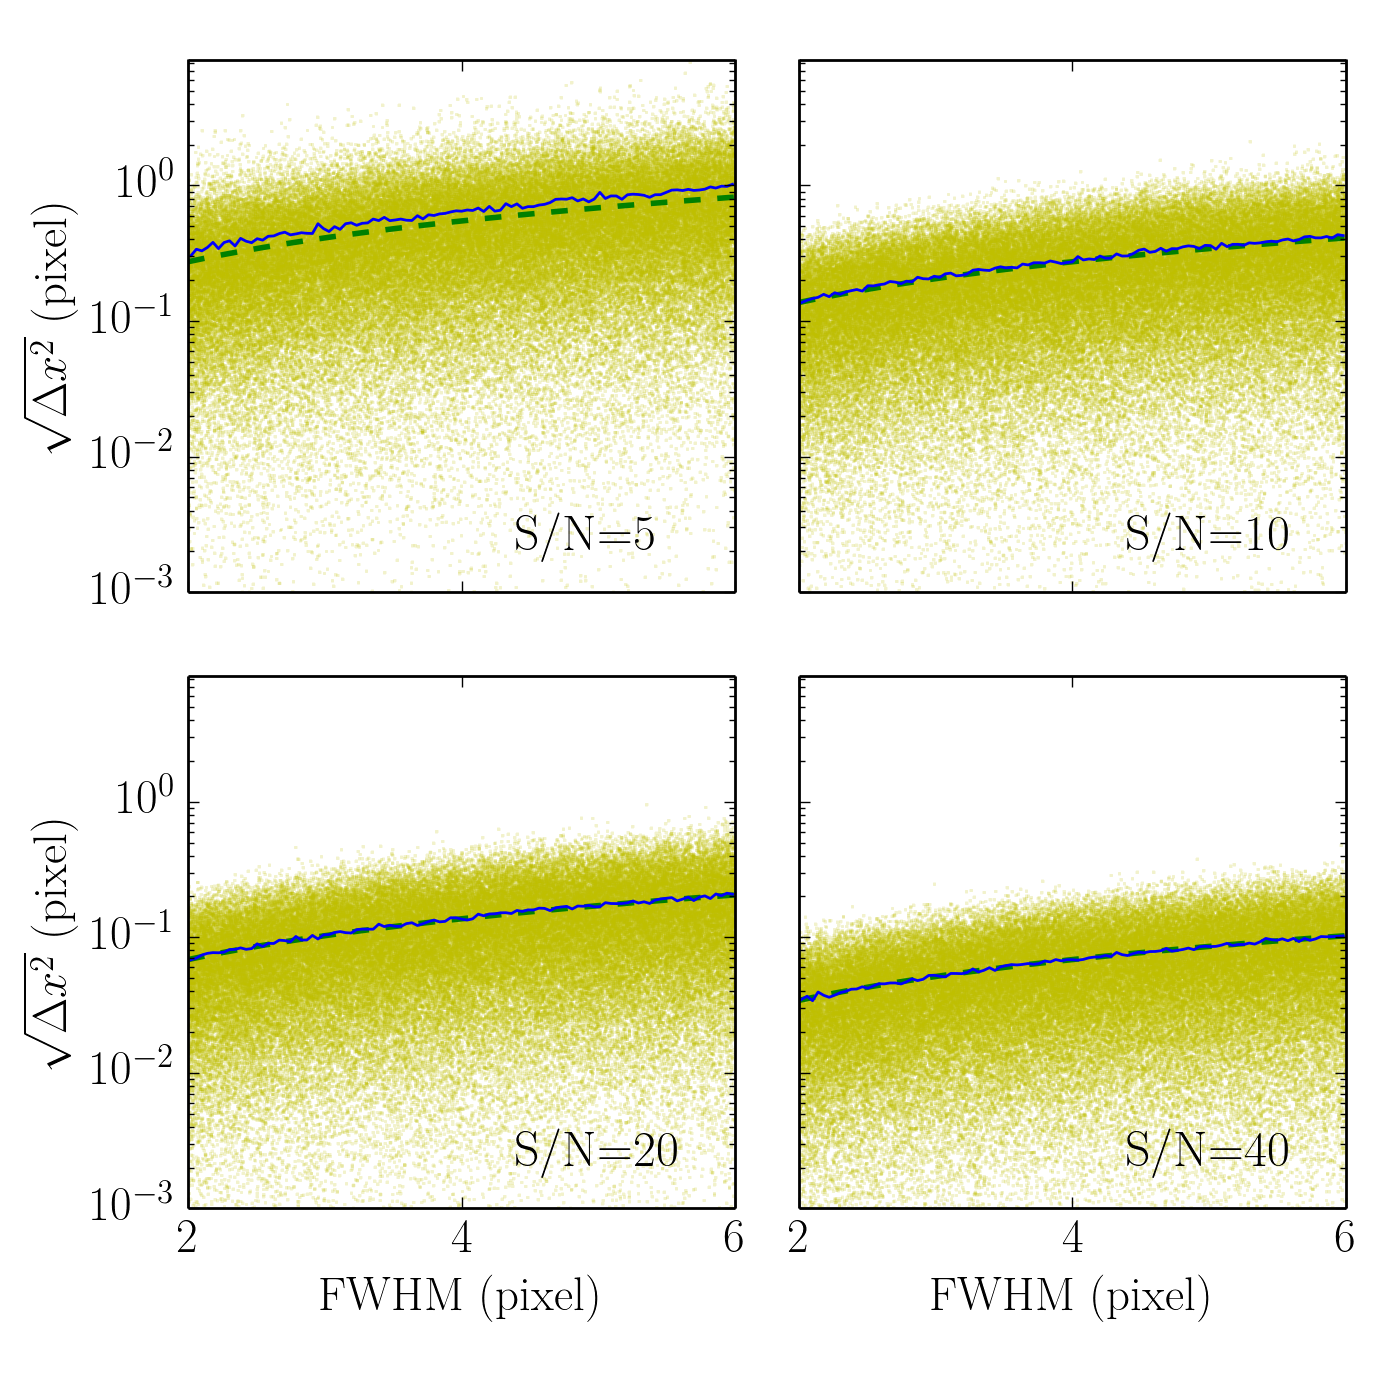
\includegraphics[width=\linewidth]{fwhm_psf.png}
\endminipage
\caption{Scatter plots showing the relation between error in centroid measurement from fitting the exact PSF model and FWHM of stars, with SNR  of : 5 (upper left), 10 (upper right), 20 (lower left), and 40 (lower right). In each scatter plot, the blue line represents the running median of data points, and the green line represents CRLB.}\label{9}
\end{figure}

\begin{figure}[!htb]
\minipage{.8\textwidth}
  \includegraphics[width=\linewidth]{fwhm_wrongpsf.png}
\endminipage
\captionScatter plots showing the relation between error in centroid measurement from fitting a Gaussian PSF model and FWHM of stars, with SNR  of : 5 (upper left), 10 (upper right), 20 (lower left), and 40 (lower right). In each scatter plot, the blue line represents the running median of data points, and the green line represents CRLB.}\label{10}
\end{figure}

\end{document}
